%%%%           %%%%
%%%% ANÁLISIS  %%%%
%%%%           %%%%

\chapter{Análisis}
\label{chap:analisis}

\lettrine{E}{n} este capítulo se tratará los aspectos del análisis de la aplicación. Se verán los requisitos, funcionales y no funcionales, los casos de uso y por último se presentarán los modelos de los documentos tratados.

\section{Actores y casos de uso}

Un caso de uso describe una interacción en entre un rol y el sistema. O cómo es utilizado por un usuario para completar una tarea u alcanzar un objetivo. En el diagrama \ref{fig:casos-de-uso} se presentan los casos de uso de la aplicación. 

Existen dos actores que interactúan con la aplicación, un sistema externo y una base de datos:

\begin{itemize}
	\item \textbf{Sistema externo}: la aplicación está diseñada para comunicarse con sistemas externo mediante invocación directa de comandos o bien un API REST. Si bien mediante comandos un usuario podrían solicitar la ejecución de trabajos en el engine, el objetivo principal es ser un backend conectado empleado por otros sistemas.
	\item \textbf{Base de datos}: este agente es consultado para la obtención de datos de idenficación de los documentos.
\end{itemize}

Se presentan a continuación los casos de uso de forma detallada:

\begin{itemize}
	\item \textbf{CU-01} - Registrar nuevo trabajo
	\begin{itemize}
		\item \textbf{Descripción}: el sistema externo solicita la generación de un nuevo identificador para un trabajo.
		\item \textbf{Precondición}: el motor está operativo y esperando trabajo.
		\item \textbf{Postcondición}: se genera el identificador y se ha creado la ruta correspondiente en el sistema de ficheros para el trabajo.
	\end{itemize}
\item \textbf{CU-02} - Generar JSON
	\begin{itemize}
		\item \textbf{Descripción}: el sistema externo facilita un lote de ficheros y un identificador del trabajo para comenzar su tratamiento.
		\item \textbf{Precondición} el identificador debió ser creado previamente.
		\item \textbf{Postcondición}: los resultados de la operativa están disponibles en las rutas previstas.
\end{itemize}
\item \textbf{CU-03} - Generar imágenes
	\begin{itemize}
		\item \textbf{Descripción}: el sistema genera imágenes para cada una de las páginas de los documentos.
		\item \textbf{Precondición} se han podido recuperar los PDF individuales y se encuentran en las rutas previstas.
		\item \textbf{Postcondición}: existe un fichero para cada página de cada documento.
\end{itemize}
\item \textbf{CU-04} - Informar error
	\begin{itemize}
		\item \textbf{Descripción}: en caso de problemas durante el procesamiento se informa al sistema externo del error ocurrido.
		\item \textbf{Precondición} sucece una condición de error en el sistema.
		\item \textbf{Postcondición}: dependiendo del tipo de error el engine consigue finalizar el procesamiento o se finaliza si no es posible recuperarse del error.
\end{itemize}
\item \textbf{CU-05} - Relacionar documento y plantilla
	\begin{itemize}
		\item \textbf{Descripción}: a partir de los datos extraídos del documento en curso se consigue identificar la plantilla correcta para la generación de su lenguaje intermedio y su posterior proceso de parseo. La búsqueda del identificador se solicita a una base de datos externa.
		\item \textbf{Precondición} los datos extraidos son de la suficiente calidad para contener el identificador del documento.
		\item \textbf{Postcondición}: se genera un fichero con el identificador único de la plantilla.Precondición
\end{itemize}
\item \textbf{CU-06} - Identificar la finalización
	\begin{itemize}
		\item \textbf{Descripción}: al finalizar el procesamiento del lote de ficheros se genera una marca de finalización del trabajo.
		\item \textbf{Precondición} se completa el tratamiento de todos los documentos sin errores mayores.
		\item \textbf{Postcondición}: la marca de finalización está en la ruta preestablecida del sistema de ficheros.
\end{itemize}

\end{itemize}

\begin{figure}[hp!]
	\centering
	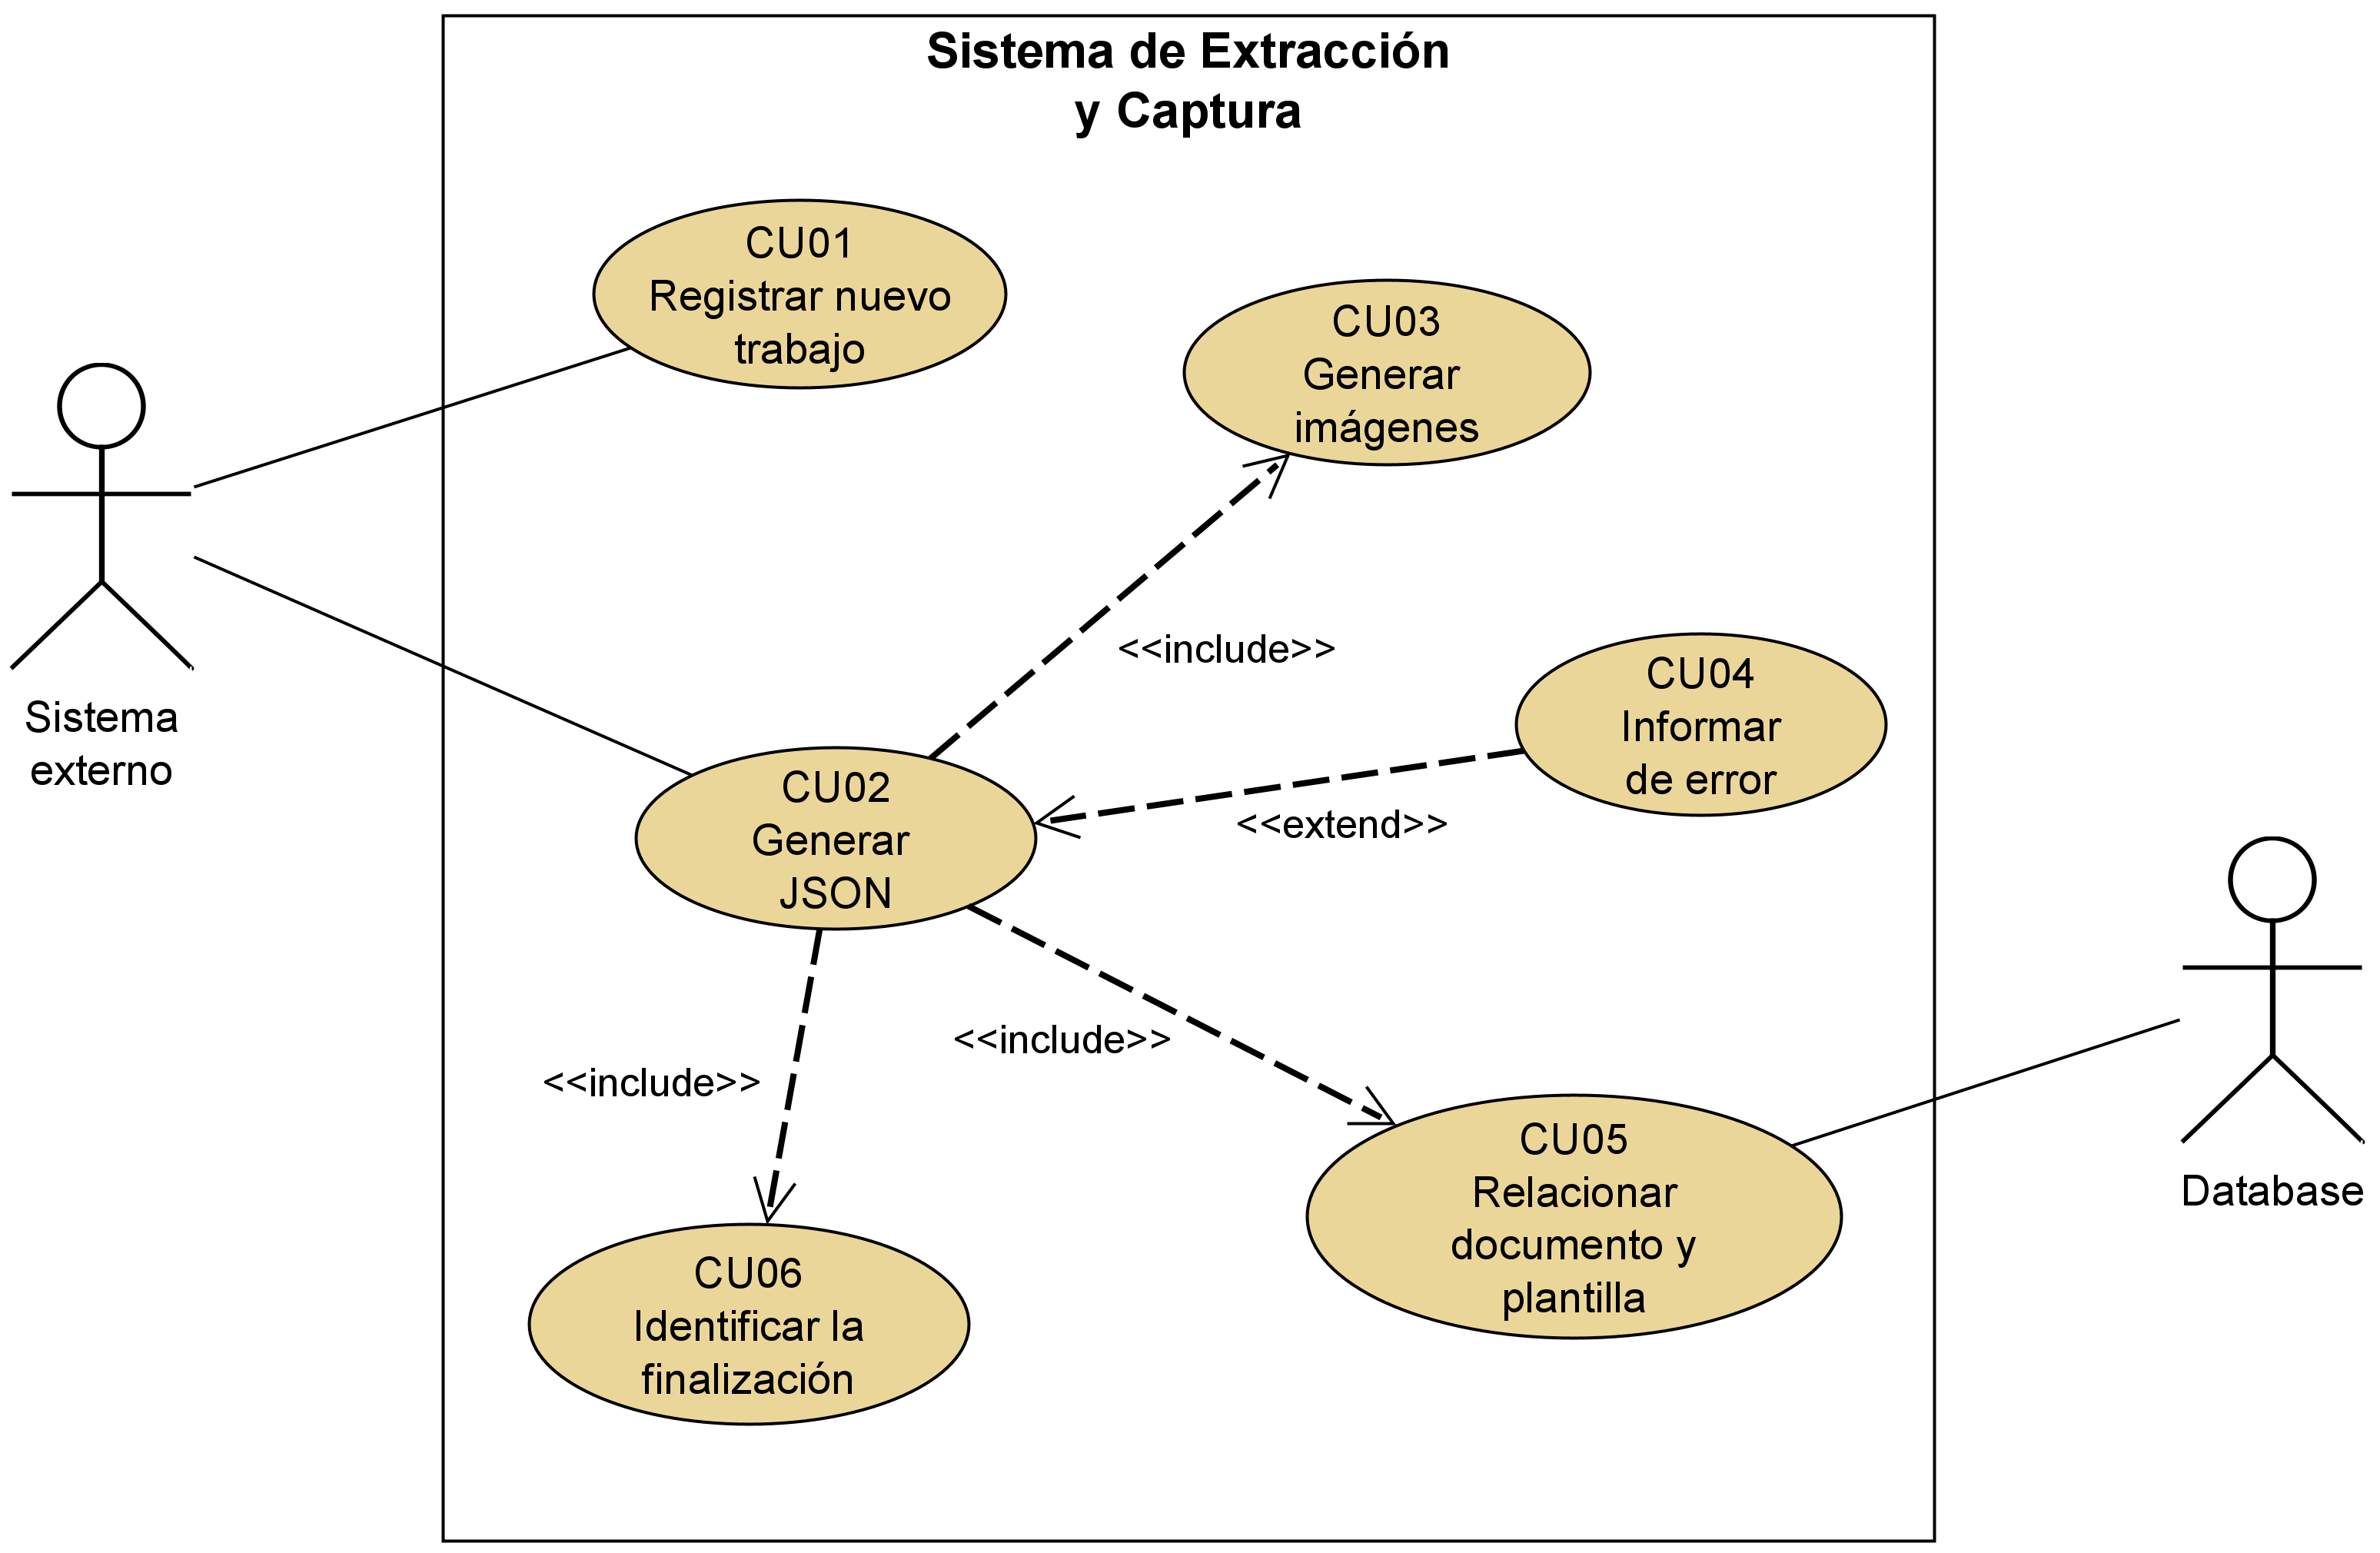
\includegraphics[width=1.0\textwidth]{imaxes/g-analisis/casos-uso.png}
	\caption{Casos de uso de la aplicación}
	\label{fig:casos-de-uso}
\end{figure}

\section{Requisitos funcionales}

Estos son los requisitos funcionales que la aplicación debe soportar:

\begin{itemize}
	\item Obtención de un identificador único de un trabajo, con anterioridad a la ejecución del mismo.
	\item Generación una salida en formato estructurado para cada documento suministrado y reconocido en el sistema.
	\item Creación de imágenes de las páginas individuales de cada uno los documentos.
	\item Creación de una marca de finalización para cada trabajo completado.
\end{itemize}


\section{Requisitos no funcionales}

Se exponen ahora los requisitos no funcionales de la aplicación:

\begin{itemize}
	\item La entrada podrá contener uno o más ficheros para su tratamiento en el mismo lote.
	\item Procesamiento de los modelos de imagen y texto de forma transparente al usuario.
	\item La salida de una ejecución debe facilitar los resultados de forma individualizada para cada documento.
	\item Se deben poder identificar las líneas individuales de las tablas existentes en los documentos.
\end{itemize}

\section{Sobre los documentos}

Se dispone de varios modelos de facturas tanto de casos basados en imagen como otros basados en texto. Estas facturas proporcionan tipos de regiones de interés que se desean capturar.

\subsection{Tipos de regiones}

\begin{enumerate}
	\item Tablas simples de dos columnas y una cabecera en la columna de la derecha.
	\item Tablas simples con una cabecera en la primera fila.
	\item Celdas individuales donde el contenido se captura de forma secuencial.
	\item Tablas con $n\times m$ dimensiones y cabecera en la primera fila.
	\item Combinación de regiones simples, como en el caso de los documentos de OVH.
\end{enumerate}

Los ejemplos de documentos basados en texto son tres

\begin{itemize}
	\item Adobe.
	\item OVH.
	\item Prodware.
\end{itemize}

% TODO añadir imagen de conjunto con los tres tipos de modelos basados en texto

% TODO añadir imagen de conjunto con los tipos de modelos basados en imagen

\subsection{Características para la identificación}

Datos para identificar los documentos. En este caso, NIF, CIF.

% TODO valorar si comentar los distintos tipos de lineas presentes en los documentos
